\documentclass{standalone}
\usepackage{tikz}
\usetikzlibrary{arrows,positioning,shapes.geometric}
\begin{document}
    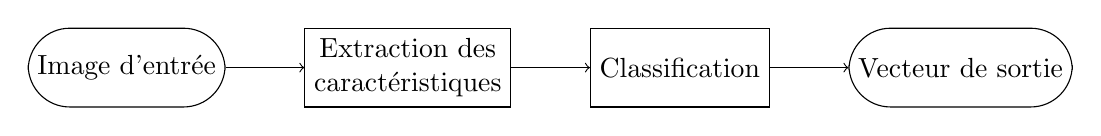
\begin{tikzpicture}
        \tikzset{block/.style= {draw, rectangle, align=center,minimum width=2cm,minimum height=1cm},
        rblock/.style={draw, shape=rectangle,rounded corners=1.5em,align=center,minimum width=2cm,minimum height=1cm},
        input/.style={ % requires library shapes.geometric
        draw,
        trapezium,
        trapezium left angle=60,
        trapezium right angle=120,
        minimum width=1cm,
        align=center,
        minimum height=1cm
    },
        }
        \node [rblock]  (start) {Image d'entrée};
        \node [block, right =1cm of start] (acquire) {Extraction des \\ caractéristiques};
        \node [block, right =1cm of acquire] (rgb2gray) {Classification};
        \node [rblock, right =1cm of rgb2gray] (otsu) {Vecteur de sortie};
        

%% paths
        \path[draw,->] (start) edge (acquire)
                    (acquire) edge (rgb2gray)
                    (rgb2gray) edge (otsu);
    \end{tikzpicture}
\end{document}